\documentclass[tikz,border=9pt]{standalone}
\usepackage{amsmath,amssymb}
\usetikzlibrary{arrows.meta,positioning,calc}
\begin{document}
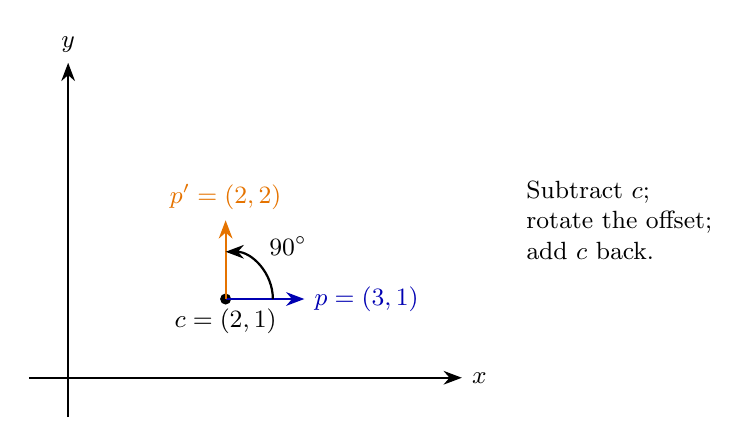
\begin{tikzpicture}[font=\small,arr/.style={-{Stealth},thick},box/.style={draw=blue!55!black,rounded corners,fill=blue!4,align=center,text width=2.9cm,minimum height=1.05cm}]

\draw[arr] (-.5,0)--(5,0) node[right]{$x$};\draw[arr] (0,-.5)--(0,4) node[above]{$y$};
\coordinate (c) at (2,1);\coordinate (p) at (3,1);\coordinate (q) at (2,2);
\fill (c) circle(2pt) node[below]{$c=(2,1)$};
\draw[arr,blue!70!black] (c)--(p) node[right]{$p=(3,1)$};
\draw[arr,orange!90!black] (c)--(q) node[above]{$p'=(2,2)$};
\draw[arr] (2.6,1) arc (0:90:.6) node[midway,above right]{$90^\circ$};
\node[align=left] at (7,2){Subtract $c$;\\rotate the offset;\\add $c$ back.};

\end{tikzpicture}
\end{document}
